% !TEX root = tesis.tex

\chapter{Mirando al Sol invisible}
\chaptermark{Aceleración de partículas}
\label{chap:uno}

Nuestra especie, por medio de sus sentidos, es consciente del mundo a su alrededor y no obstante; ha invertido miles de años en tratar de entender aquello que con los sentidos podemos percibir, usando la razón. Comprender el espacio en el que habitamos y las complejas relaciones entre sus diversos elementos representa una de las más altas aspiraciones de la raza humana.

Así, con nuestros ojos vemos a través de la luz sin poder entender completamente su naturaleza y origen. Hoy nuestra compresión del fenómeno es ligeramente superior, no solo gracias al desarrollo de complejos modelos teóricos, sino a la construcción de instrumentos que nos permiten observar más allá de nuestro sentir.

El descubrimiento de la radiación de fondo de microondas (\emph{CMB} por su siglas en inglés) constituye uno de nuestros más grandes hallazgos, en ella se encuentran las evidencias de nuestro origen: fotones provenientes del \emph{big bang} corridos hacia la banda de microondas en su largo viaje desde los rincones del universo en expansión. A gran escala, el \emph{CMB} es isotrópico pues el universo no tiene una dirección preferente para su evolución. Son sin embargo las diminutas fluctuaciones en su espectro la característica más impactante, ya que brindan la evidencia necesaria para la formación de materia y galaxias a partir de los hechos ocurridos hace miles de millones de años.

\section{Ráfagas solares}

Las ráfagas solares (también conocidas como fulguraciones) son fenómenos explosivos que se observan en la atmósfera del Sol, la cual está llena de plasma magnetizado. La energía que se libera durante una ráfaga se encuentra en el rango de \SI{e28}{erg} a \SI{e32}{erg} y puede emitirse en diferentes productos. La magnitud espacial de las cuerdas magnéticas de la ráfaga va desde los \SI{e4}{\metre} hasta los \SI{e5}{\metre}, aunque varia de evento a evento. El tamaño afecta directamente la duración (entre \SI{e3}{\second} y \SI{e4}{\second}) y la cantidad de energía liberada.

Las ráfagas se observan en un amplio rango del espectro electromagnético; en ondas de radio, radiación óptica, rayos \emph{X} y rayos $\gamma$. La figura \ref{fig:flare-euv} muestra un ejemplo de la observación una ráfaga por medio del satélite \emph{SDO} (Solar dynamics observatory), ocurrida el \num{19} de Julio de \num{2012} (la explicación detallada de la imagen se da más adelante). Por otro lado, las explosiones puede acelerar iones y electrones a energías relativistas; que a su vez pueden producir otras partículas. De forma cualitativa podemos clasificar e las fulguraciones en cinco grupos de acuerdo a la intensidad de la emisión de rayos \emph{X}, la cual es indicativa de la cantidad de energía que radia el plasma coronal. Para la clasificación grupos se usa la banda de \SI{0.1}{\nano\metre} a \SI{0.8}{\nano\metre} del satélite \emph{GOES}, localizado a una distancia de \SI{1}{AU}. La clasificación es la siguiente: \emph{A}(\SI{\geq e-8}{\watt\per\square\metre}), \emph{B}(\SI{\geq e-7}{\watt\per\square\metre}), \emph{C}(\SI{\geq e-6}{\watt\per\square\metre}), \emph{M}(\SI{\geq e-5}{\watt\per\square\metre}) y \emph{X}(\SI{\geq e-4}{\watt\per\square\metre}).

La enorme cantidad de energía liberada durante la explosión puede explicarse a través de los modelos de reconexión magnética, propuestos originalmente entre \num{1946} y \num{1958} \cite{giovanelli,hoyle,sweet,parker}. En estos modelos, cuerdas de flujo magnético (tubos de flujo torcidos) emergen a la superficie solar debido al efecto de boyancia originado por las diferencias de densidad entre el plasma del tubo y su alrededor. Una vez que las cuerdas se encuentra en la superficie, su campo magnético es comprimido por el plasma en su vecindad que se mueve a una cierta velocidad. El resultado de la compresión crea zonas en donde interaccionan lineas de campo de polos opuestos y en el punto neutro surge una hoja de corriente. Eventualmente el flujo de corriente produce un gradiente del campo magnético y la topología se reorganiza para encontrar una configuración de menor energía \cite{shiba11}. A través de este proceso, la energía magnética almacenada en el hoja de corriente se convierte en energía cinética y térmica; además de estar acompañada de intensos campos eléctricos los cuales pueden ser los responsables de la aceleración de partículas.

La existencia del proceso de reconexión magnética fue comprobada mediante observaciones en rayos \emph{X} del satélite \emph{Youkou} \cite{masuda,tsuneta} y simulaciones magnetohidrodinámicas de la atmósfera solar  \cite{yokoyama}; sin embargo se necesitan observaciones más detalladas para confirmar los modelos. Otro avance importante en la compresión de los fenómenos solares se dio en Julio de \num{2012}, con la observación por parte del satélite SDO de la formación de cuerdas magnéticas. La figura \ref{fig:flare-euv} muestra la evolución temporal de una ráfaga ocurrida el dia \num{19}. En el panel superior izquierdo se observa el lapso de tiempo antes de la explosión, a una longitud de onda de \SI{17}{\nano\metre}, la cual sirve para observar la corona solar en estado de reposo. El panel superior derecho muestra el mismo evento minutos después; en la parte derecha de la imagen se aprecia una zona que se ilumina ligeramente naranja. La intensa emisión en tres bandas de EUV (radiación ultravioleta extrema) está asociada con los intensos campos magnéticos de la cuerda. Los paneles inferiores fueron registrados \SI{8}{\hour} después, cuando la compleja estructura del campo magnético se reorganiza dando lugar a la ráfaga.

\begin{figure}
        \centering
        \begin{subfigure}[b]{0.49\textwidth}
                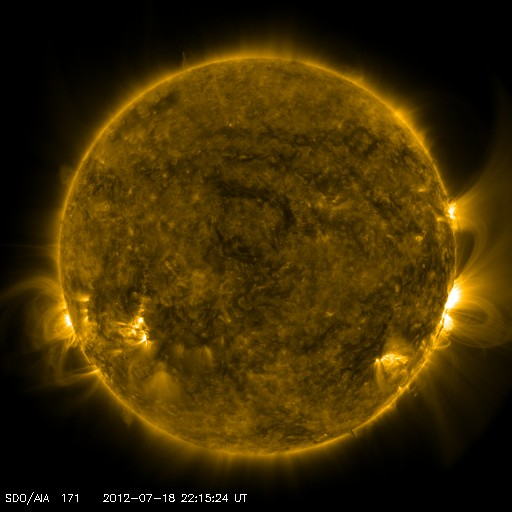
\includegraphics[width=7.25cm]{sdo120718-2215-17}
                \caption*{Imagen en la banda de \SI{17}{\nano\metre}.}
        \end{subfigure}
        \begin{subfigure}[b]{0.49\textwidth}
                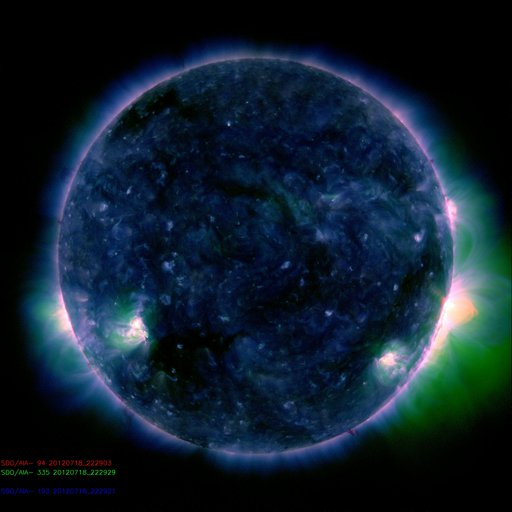
\includegraphics[width=7.25cm]{sdo120718-2229-c}
                \caption*{Imagen compuesta: \SI{9}{\nano\metre}, \SI{19}{\nano\metre} y \SI{33}{\nano\metre}.}
        \end{subfigure}
        \begin{subfigure}[b]{0.49\textwidth}
                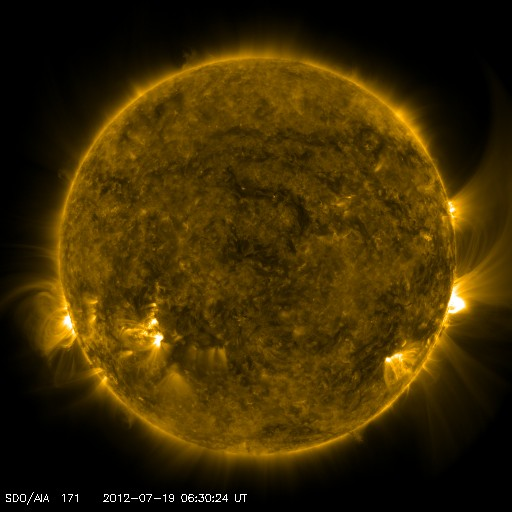
\includegraphics[width=7.25cm]{sdo120719-0630-17}
                \caption*{Imagen en la banda de \SI{17}{\nano\metre}.}
        \end{subfigure}
        \begin{subfigure}[b]{0.49\textwidth}
                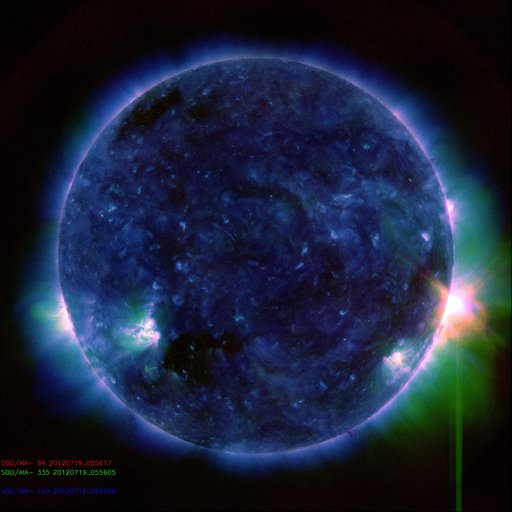
\includegraphics[width=7.25cm]{sdo120719-0555-c}
                \caption*{Imagen compuesta: \SI{9}{\nano\metre}, \SI{19}{\nano\metre} y \SI{33}{\nano\metre}.}
        \end{subfigure}
        \caption{Imágenes tomadas por el SDO durante la ráfaga del \num{19} de Julio de \num{2012}. Los paneles superiores presentan la formación de una cuerda magnética \SI{8}{\hour} antes del evento. Los paneles inferiores registran el momento de la posible reconexión magnética. Fuente: \url{https://sdo.gsfc.nasa.gov}}
        \label{fig:flare-euv}
\end{figure}

\section{Aceleración de partículas en Ráfagas}

La primera evidencia de aceleración que el Sol podía acelerar partículas a energías relativistas (iones y electrones) se observó en \num{1942}

The first evidence of acceleration of charged particles (electrons and ions) to relativistic en-
ergies in association with solar flares was found in 1942 with the discovery of large increases
in the count rates of several ground level cosmic-ray intensity monitors. These observations
told us, more than fifty years ago, that solar flares are capable of accelerating protons to
GeV energies

\begin{figure}
        \centering
        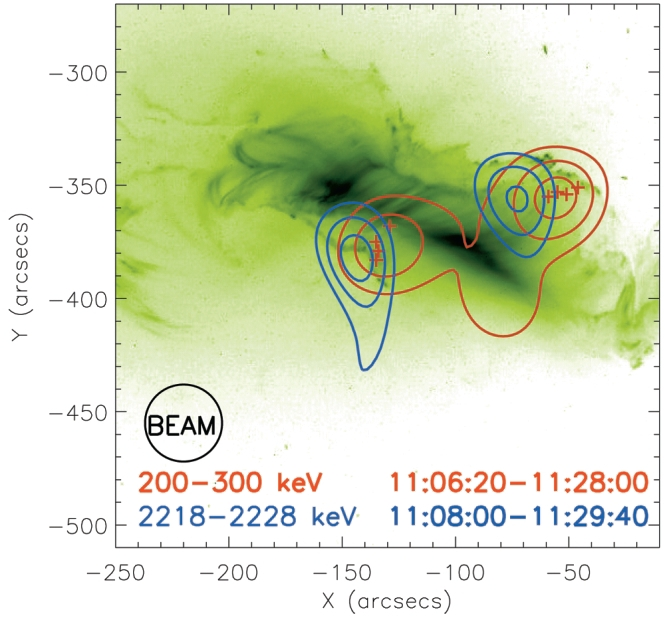
\includegraphics[width=0.75\textwidth]{flare-footprints}
        \caption{Imagen compuesta de observaciones en rayos \emph{X} y $\gamma$ de la ráfaga solar ocurrida el \num{28} de Octubre de \num{2003}. Los contornos azules y rojos muestran la zona donde se aceleran la partículas dentro de la región activa que produjo la ráfaga.}
        \label{fig:flare-foot}
\end{figure}


\section{Propagación de neutrones solares}

Cuando los neutrones escapan de la atmósfera solar viajan sin ser afectados por los campos magnéticos en el medio interplanetario. Los neutrones libres son inestables y están sujetos a decaimiento $\beta$ con una vida media de $\tau=\SI{880.3}{\second}$. Debido a esto, el espectro de neutrones que arriban a la orbita terrestre se modifica, afectando principalmente a los neutrones de baja energía. Para tener un modelo cuantitativo de este efecto usaremos la siguiente expresión; la probabilidad de que una partícula con $\tau$ tiempo de vida media, sobreviva y alcance la Tierra sin decaer:

\begin{equation}
P\left(E_{k},r\right)=\exp\left(-\frac{t}{\gamma\tau}\right)
\end{equation}

en donde $E_{k}$ es la energía cinética de la partícula, $r$ es la distancia a la fuente (para neutrones solares $r=\SI{1}{AU}$), $t$ es el tiempo de vuelo de la partícula y $\gamma$ es factor de Lorentz. Denominaremos $P(E_{k},1AU)$ como la probabilidad de arribo de neutrones. Para neutrones con energías cinéticas $E_{k}=\SI{100}{\mega\electronvolt}$ el tiempo de vuelo es de aproximadamente \SI{1165}{\second}, con lo cual decaen el \SI{70}{\percent} de las partículas emitidas. Luego entonces, los neutrones solares con esta energía pueden ser detectados en el espacio o en superficie. Un aspecto interesante es que los productos del decaimiento (protones y electrones) también se observan, siempre y cuando son logren distinguir de la emisión de protones solares; lo cual se ha reportado con anterioridad --citas.

El panel de la izquierda en la figura \ref{fig:neutron-prob} muestra la probabilidad de arribo de neutrones en el rango de energías de \num{10}-\SI{1000}{\mega\electronvolt}. La utilidad de esta gráfica viene de que puede ser utilizada como función de respuesta para corregir el espectro de energías de neutrones solares observado en el Tierra. Como se observa en la figura, en principio es posible detectar neutrones de bajas energías, sin embargo más adelante veremos que la principal limitante es la atenuación atmosférica. El panel de la derecha muestra el tiempo de vuelo en función de la energía cinética de los neutrones.

\begin{figure}
        \centering
        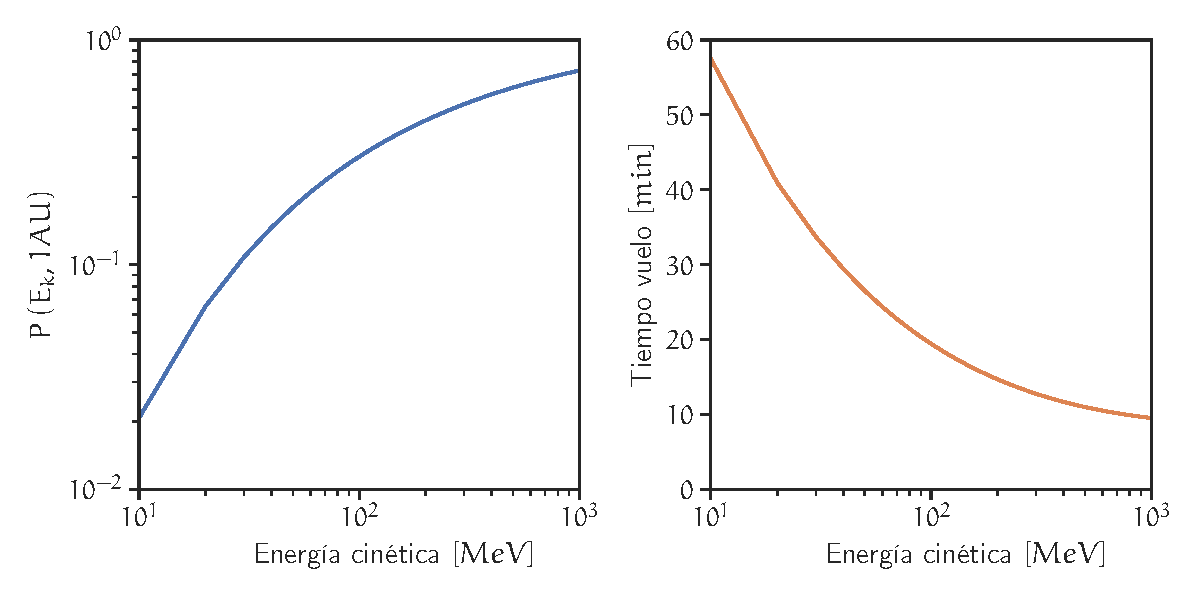
\includegraphics[width=\textwidth]{neutron-prob.pdf}
        \caption{Probabilidad de arribo de neutrones solares a la orbita terrestre (panel izquierdo) y tiempo de vuelo (panel derecho).}
        \label{fig:neutron-prob}
\end{figure}

Los neutrones que inciden al tope de la atmósfera terrestre, se propagan hacia la superficie colisionando en el trayecto con núcleos atmosféricos. Durante el trayecto, tres procesos importantes ocurren: dispersión elástica, dispersión inelástica e intercambio de carga.

El proceso de dispersión elástica es el único que contribuye de manera positiva a la propagación de neutrones ya que la transferencia de energía de los neutrones a los núcleos atmosféricos es limitada en núcleos de Oxigeno y Nitrógeno (máximo $0.22$ de la energía incidente en el caso del Oxigeno y $0.28$ para el caso del Nitrógeno). Luego entonces, es de esperarse que la mayoría de los neutrones sujetos a este proceso lleguen a altitudes de alta montaña; no obstante con modificaciones en el espectro de energía y distribución angular. Los dos procesos restantes contribuyen a la atenuación de los neutrones solares. En el proceso de intercambio de carga los neutrones interaccionan con núcleos atmosféricos y en su lugar se emiten protones en la dirección frontal. En este caso la transferencia de energía es casi total y los protones emitidos son absorbidos en la atmósfera mediante ionización. Por otro lado, en la dispersión inelástica los neutrones proyectiles transfieren energía a los núcleos dejándolos en un estado excitado y generando una gran cantidad de productos secundarios (entre ellos neutrones secundarios). De manera general la dispersión inelástica contribuye de manera importante a la atenuación de los neutrones, no obstante sus productos pueden ser observados a cierta profundidad atmosférica \cite{shibata94}.

La figura \ref{fig:neutron-at} muestra el resultado de una simulación monte carlo (MC) de la propagación de \num{e8} neutrones solares en la atmósfera terrestre. Para realizar la simulación utilicé el modelo de Shibata \cite{shibata94}, el cual permite estudiar el espectro de los neutrones solares a diferentes profundidades atmosféricas y además ha sido calibrado con experimentos en aceleradores de partículas. En el modelo, los neutrones se inyectan al tope de la atmósfera, con un ángulo cenital definido (para nuestro caso $\theta=0$) y un índice espectral. Como se aprecia en la figura la mayor atenuación la sufren los neutrones de baja energía, independientemente de la profundidad, volviéndose factible detectar neutrones solares a partir de \SI{100}{\mega\electronvolt}. Por otro lado, también es posible estudiar los efectos de la atenuación en función de una profundidad especifica. De la figura se puede concluir, que las localidades de alta montaña tienen características apropiadas para la observación de neutrones.

\begin{figure}
        \centering
        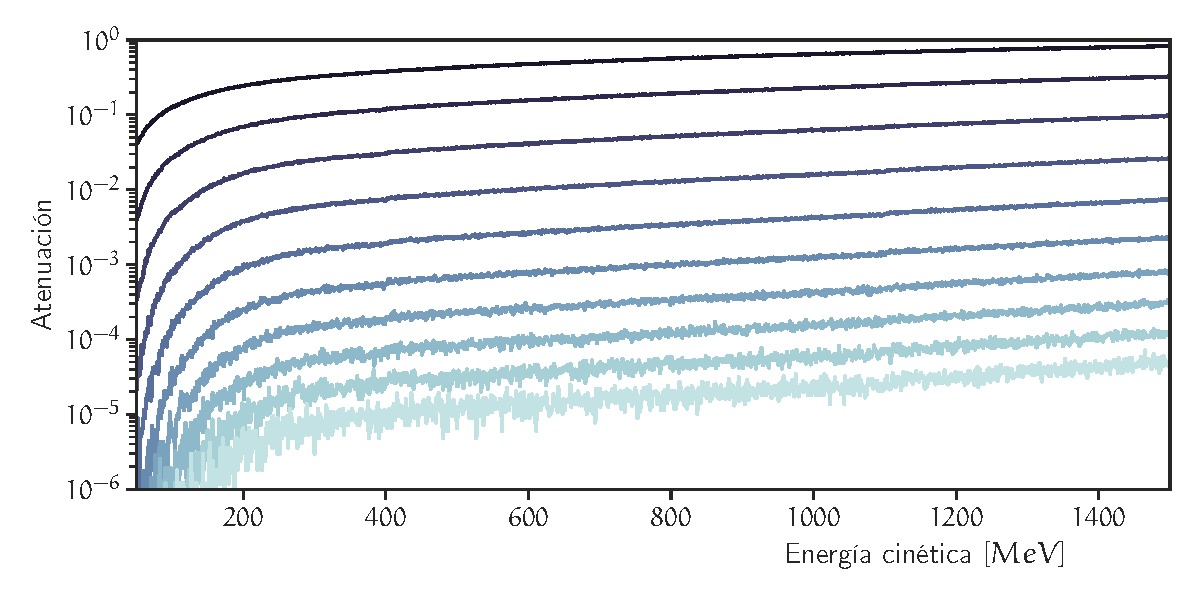
\includegraphics[width=\textwidth]{neutron-at.pdf}
        \caption{Simulación MC de la atenuación de neutrones solares en función de la energía cinética al tope de la atmósfera y profundidad atmosférica. Del color más oscuro al más claro, la profundidad atmosférica varia de \SI{100}{\gram\per\square\cm} a \SI{1000}{\gram\per\square\cm}.}
        \label{fig:neutron-at}
\end{figure}

Otra característica importante a estudiar es el perfil temporal de los neutrones cuando arriban a una cierta localidad, el cual está directamente relacionado con su espectro de energía. En la figura \ref{fig:neutron-time} muestro el resultado de simular neutrones con diferentes índices espectrales (entre \num{3.0} y \num{5.0}) arribando a la profundidad de Sierra Negra (\SI{575}{\gram\per\cm\square}). Como es de esperarse, al incrementar el índice espectral, los neutrones de menor energía se vuelven más dominantes en el espectro y por lo tanto, el tiempo de vuelo de los neutrones emitidos por el Sol se ve retardado. Es propiedad de los neutrones nos permite diferenciar entre distintos mecanismos de aceleración.

\begin{figure}
        \centering
        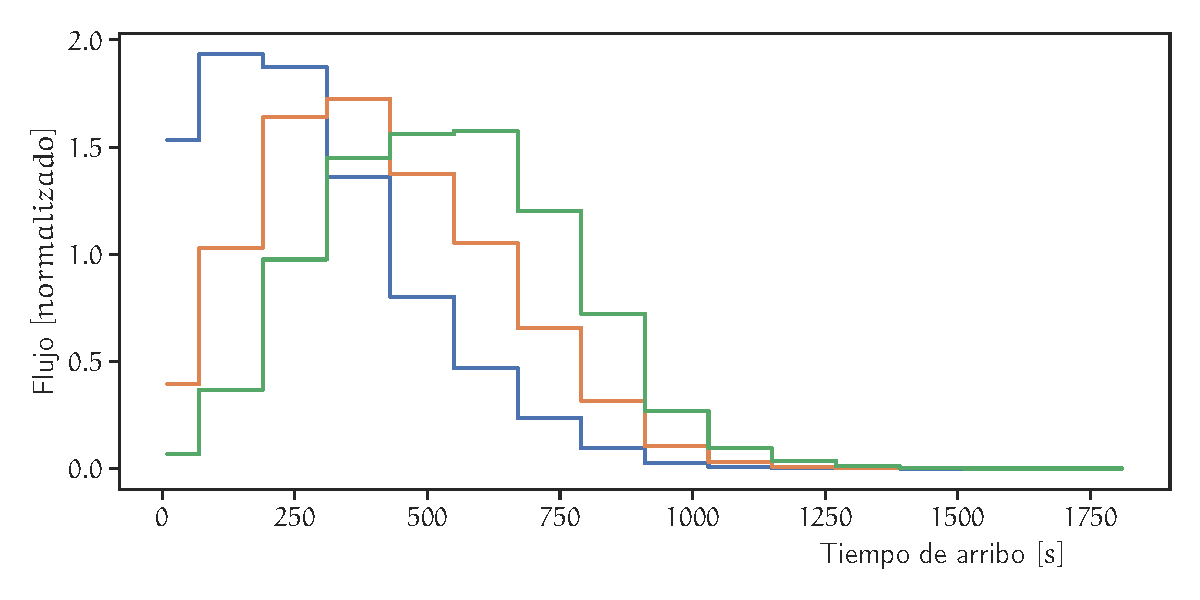
\includegraphics[width=\textwidth]{neutron-time.pdf}
        \caption{Perfiles temporales del arribo de neutrones en función del índice espectral $\alpha$. En azul $\alpha=3.0$, naranja $\alpha=4.0$ y verde $\alpha=5.0$.}
        \label{fig:neutron-time}
\end{figure}

\section{Observaciones de neutrones solares}
